\begin{frame}[fragile]{OpenMP}
    \begin{columns}[T]
        \begin{column}{0.48\textwidth}

             
            \begin{center}
                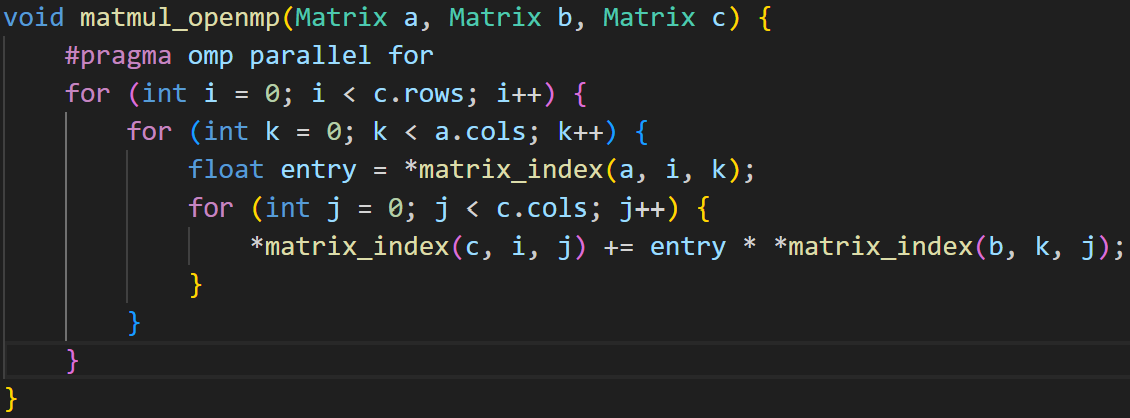
\includegraphics[width=0.99\textwidth]{Images/matmul_openmp.png}
           \end{center}
            
           \begin{itemize}
            \item hello
           \end{itemize}

            
            
        \end{column}
        
        \hfill
        \hfill
        
        \begin{column}{0.48\textwidth}
            
          \begin{itemize}
            \item hello 2
          \end{itemize}
            
        \end{column}
    \end{columns}
\end{frame}

\begin{frame}[fragile]{OpenMP}
    \begin{columns}[T]
        \begin{column}{0.48\textwidth}

             
            \begin{itemize}
                \item hello
            \end{itemize}

            
            
        \end{column}
        
        \hfill
        \hfill
        
        \begin{column}{0.48\textwidth}
            
           \begin{center}
                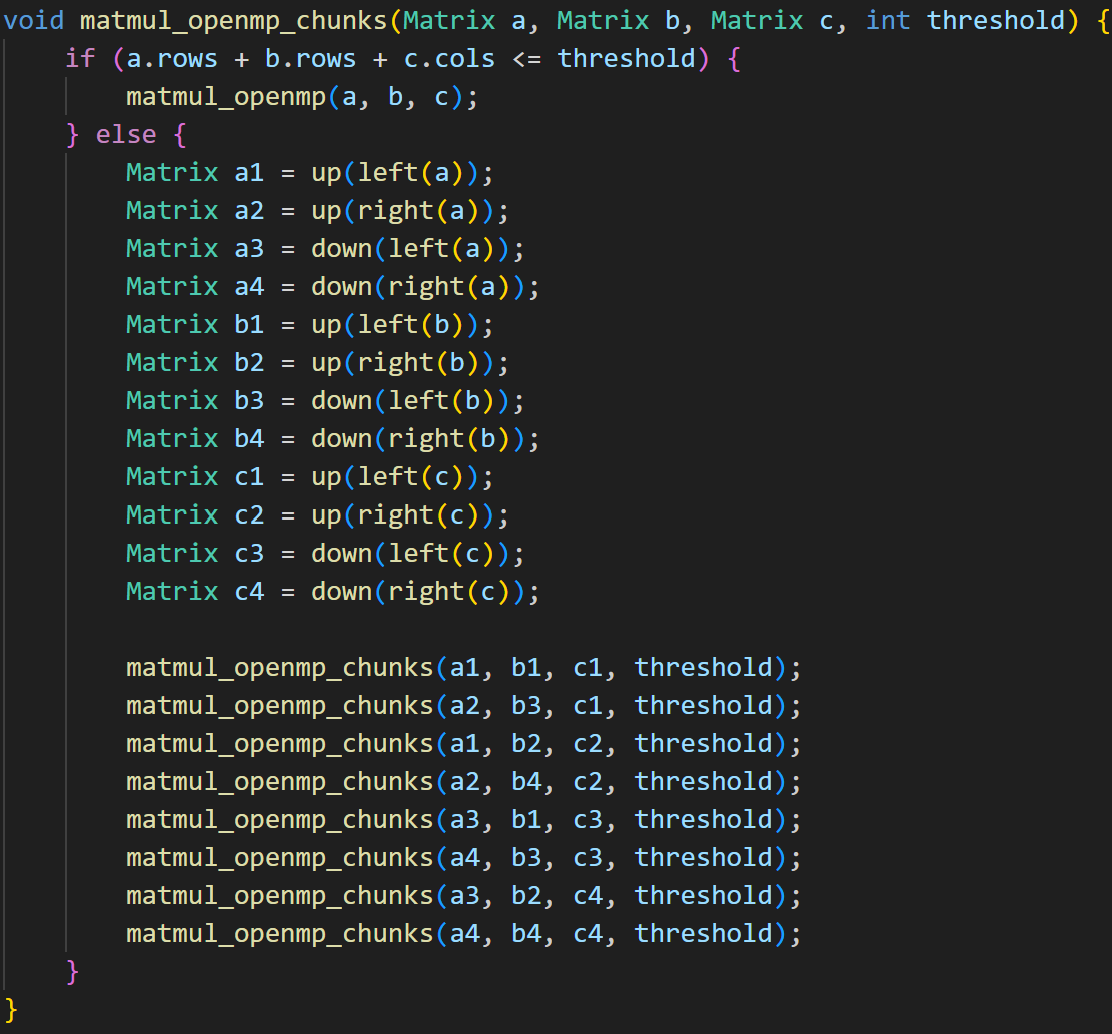
\includegraphics[width=0.99\textwidth]{Images/openmp_chunks.png}
           \end{center}
            
            
        \end{column}
    \end{columns}
\end{frame}


\begin{frame}{OpenMP}
    
    \centering
    \small
    \begin{figure}
    \begin{tabular}{lrrrr}
        \toprule
        & \multicolumn{4}{c}{\textbf{Matrix Dimension ($N \times N$)}} \\
        \cmidrule(lr){2-5}
        \textbf{Algorithm Variant} & \textbf{1024} & \textbf{2048} & \textbf{4096} & \textbf{8192} \\
        \midrule
        IKJ Loop          & 0.02 s        & 0.30 s        & 3.20 s       & 47.76 s      \\
        Transposed        & 0.11 s        & 0.81 s        & 9.01 s       & 85.15 s      \\
        Chunks            & 0.04 s        & 0.24 s        & 1.98 s       & 18.18 s      \\
        \bottomrule
    \end{tabular}
    \caption{Execution times for different OpenMP matrix multiplication algorithms, averaged over 3 consecutive runs using 12 threads.}
    \end{figure}

    \begin{itemize}
        \item A breif comment or two about the results
    \end{itemize}

    \begin{center}
        \usebeamercolor[fg]{infrastructure}
        \fontsize{6.5pt}{7.5pt}\selectfont
        \texttt{Hardware | Arch Linux \quad  11th Gen Intel(R) Core(TM) i5-11400H (6C/12T)}
    \end{center}
    
\end{frame}

